% Slides 191--200
\sectionframe{10 / Human-directed agent engineering}{The pricer and the collaborative system that built it are co-equal achievements}{Local Mac workflow; repository artifacts; official OpenAI Codex and Anthropic Claude Code documentation.}

\begin{frame}{The product was built inside a visible collaborative workspace}
  \centering
  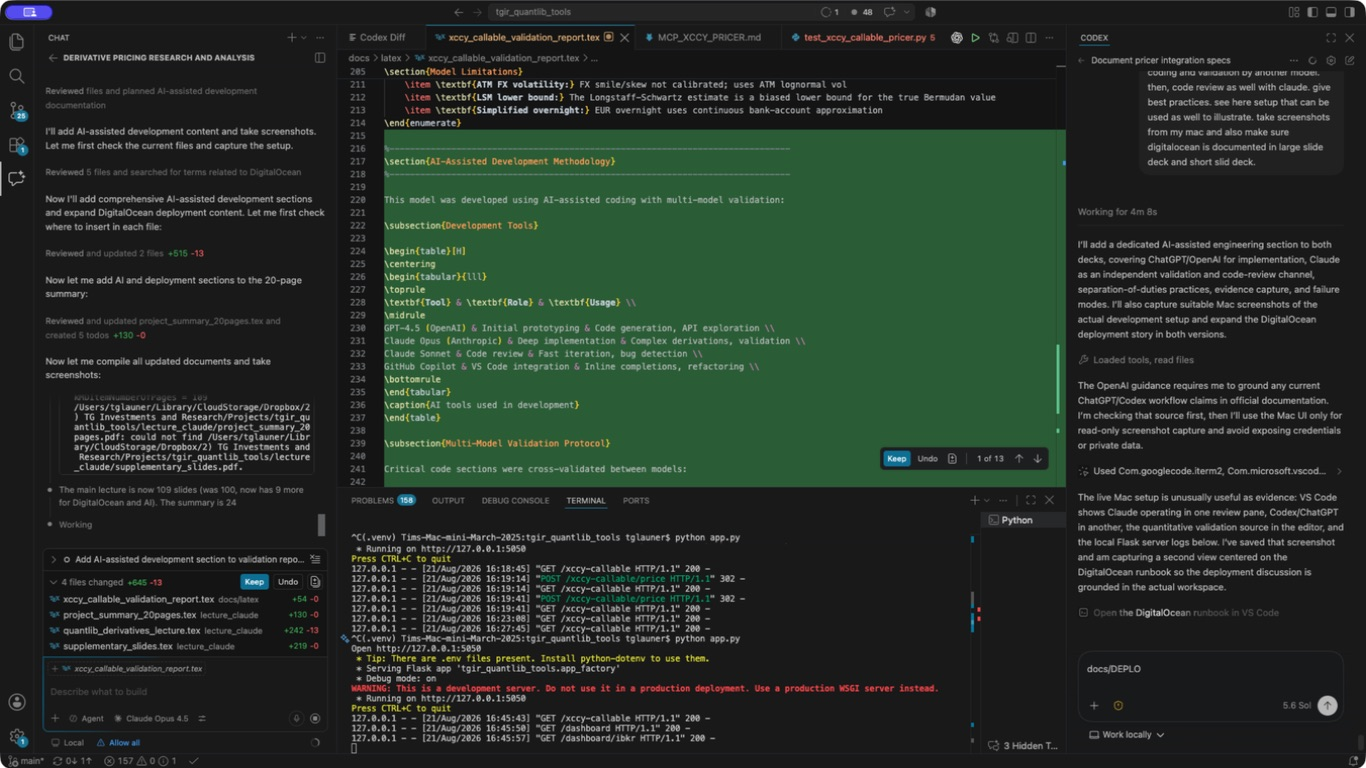
\includegraphics[height=47mm]{assets/mac_cross_model_review_setup.jpg}
  \takeaway{Tim, Codex, and Claude worked against the same inspectable Git repository, source, diffs, tests, specifications, and local server logs.}
  \src{Mac screenshot captured 2026-08-21 from the user's VS Code workspace; no secrets shown.}
\end{frame}

\lesson{The human led the work; the agents performed most of the construction}
{Tim set the economic questions, product scope, priorities, constraints, and acceptance standard, and repeatedly challenged the outputs.}
{Codex produced most foundational specifications, implementation, integration code, documentation, and executable tests.}
{Claude reviewed the Codex work and then built extensions around it for independent validation, regression testing, and future-change protection.}
{This was human-directed engineering by two active coding agents, not autocomplete and not a human manually transcribing generated snippets.}
{User development record; repository files and tests; local Codex and Claude workspace sessions.}

\lesson{Codex was the primary specification and programming agent}
{Codex translated conversational requirements into explicit deal semantics, model dynamics, calibration objectives, LSM recursion, interfaces, and acceptance criteria.}
{It implemented the Python/QuantLib pricing core, JSON inputs, CLI, web page, editable correlation controls, MCP boundary, documentation, and deployment changes.}
{It also wrote and ran unit, integration, calibration, convergence, Greek, bump-stability, and web smoke tests, then compiled and inspected the evidence.}
{The specification, code, tests, and operating instructions were developed as one connected deliverable.}
{Repository chronology; callable XCCY specifications, implementation, tests, UI, MCP, REST notes, and deployment artifacts.}

\lesson{Claude turned review into a durable validation layer}
{Claude first reviewed frozen Codex diffs findings-first, checking quantitative correctness, event ordering, numerical methods, APIs, security, and maintainability.}
{More importantly, Claude added independent validation and regression extensions around the Codex core rather than stopping at prose comments.}
{Those executable checks preserve benchmarks, reproduce accepted defects, and challenge later changes for drift signs, calibration, martingales, convergence, and bump behavior.}
{The second agent increased the system's future reliability by converting review conclusions into repeatable controls.}
{Local Claude review work; validation reports; quantitative and application regression suites.}

\begin{frame}{One cohesive framework connects people, agents, code, and hosting}
  \centering
  \begin{tikzpicture}[node distance=3mm and 3mm,every node/.style={font=\tiny,align=center}]
    \node[draw,rounded corners,fill=TgirMint!60,minimum width=19mm,minimum height=12mm] (tim) {Tim\\economics + acceptance};
    \node[draw,rounded corners,fill=white,right=of tim,minimum width=19mm,minimum height=12mm] (codex) {Codex\\specs + core + tests};
    \node[draw,rounded corners,fill=TgirMint!60,right=of codex,minimum width=19mm,minimum height=12mm] (claude) {Claude\\review + validation};
    \node[draw,rounded corners,fill=white,right=of claude,minimum width=19mm,minimum height=12mm] (stack) {QuantLib\\Python + C++};
    \node[draw,rounded corners,fill=TgirMint!60,right=of stack,minimum width=19mm,minimum height=12mm] (cloud) {DigitalOcean\\host + health checks};
    \foreach \x/\y in {tim/codex,codex/claude,claude/stack,stack/cloud}{\draw[-{Latex},thick,TgirTeal] (\x)--(\y);}
    \draw[-{Latex},thick,TgirOrange,bend right=35] (claude.south) to node[below,font=\tiny]{regression findings} (codex.south);
    \draw[-{Latex},thick,TgirOrange,bend left=38] (cloud.north) to node[above,font=\tiny]{runtime evidence} (tim.north);
  \end{tikzpicture}
  \vspace{5mm}
  \takeaway{The Mac and Git repository are the shared engineering floor; a roughly USD 7/month DigitalOcean host makes this serious hobby continuously available.}
  \src{Repository architecture and deployment notes; local workspace; DigitalOcean workflow.}
\end{frame}

\lesson{Stack Overflow accelerated discovery but never decided correctness}
{Community discussions helped locate QuantLib wrapper behavior, constructor changes, curve-horizon issues, multi-curve limitations, and known engine boundaries.}
{Every useful suggestion was checked against the installed QuantLib version, upstream source or official documentation, and a minimal executable reproduction.}
{Product-specific conclusions---especially the absence of a native callable XCCY composition---were established from current APIs and source, not an old answer alone.}
{Community knowledge shortened the search; version-pinned source inspection and tests converted it into evidence.}
{Stack Overflow QuantLib discussions on Hull--White curves, calibration-helper renames, multi-curve swaptions, and Python bindings; QuantLib 1.43 source.}

\begin{frame}{One prompt can drive the complete delivery loop}
  \centering
  \begin{tikzpicture}[node distance=3mm and 3mm,every node/.style={font=\tiny,align=center}]
    \node[draw,rounded corners,fill=TgirMint!55,minimum width=21mm,minimum height=10mm] (prompt) {Tim's prompt};
    \node[draw,rounded corners,fill=white,right=of prompt,minimum width=21mm,minimum height=10mm] (code) {specification\\+ coding};
    \node[draw,rounded corners,fill=TgirMint!55,right=of code,minimum width=21mm,minimum height=10mm] (test) {regression\\tests};
    \node[draw,rounded corners,fill=white,right=of test,minimum width=21mm,minimum height=10mm] (browser) {browser UI\\tests};
    \node[draw,rounded corners,fill=TgirMint!55,right=of browser,minimum width=21mm,minimum height=10mm] (docs) {documentation};
    \node[draw,rounded corners,fill=white,below=8mm of docs,minimum width=21mm,minimum height=10mm] (local) {optional\\local run};
    \node[draw,rounded corners,fill=TgirMint!55,left=of local,minimum width=21mm,minimum height=10mm] (deploy) {DigitalOcean\\deployment};
    \node[draw,rounded corners,fill=white,left=of deploy,minimum width=21mm,minimum height=10mm] (remote) {remote\\regressions};
    \node[draw,rounded corners,fill=TgirOrange!25,left=of remote,minimum width=21mm,minimum height=10mm] (telegram) {Telegram\\``all done''};
    \foreach \x/\y in {prompt/code,code/test,test/browser,browser/docs,docs/local,local/deploy,deploy/remote,remote/telegram}{\draw[-{Latex},thick,TgirTeal] (\x)--(\y);}
  \end{tikzpicture}
  \vspace{3mm}
  \takeaway{After the initiating prompt, the workflow can proceed without manual handoffs; the optional local run remains available when Tim wants to inspect it personally.}
  \src{User-described operating workflow; repository tests, browser UI, documentation, and DigitalOcean assets. Telegram orchestration is external to this repository.}
\end{frame}

\lesson{Evidence and authority remain explicit across both agents}
{Freeze economic inputs and record commit, model/provider, prompt, permissions, commands, seeds, exit codes, reports, and known limitations.}
{Keep secrets and unrestricted production data away from agent context; grant edits, shell, network, deployment, commit, and push authority only when needed.}
{Require the human owner to triage findings, resolve disagreements, accept residual model risk, and authorize releases.}
{A persuasive response is not evidence; a reproducible specification, diff, benchmark, regression, and deployment check are.}
{Repository AGENTS.md; official OpenAI Codex review guidance; Anthropic Claude Code security guidance.}

\lesson{The reusable achievement is an AI-native quantitative engineering method}
{The complex three-factor callable XCCY pricer demonstrates that the method can handle coupled stochastic dynamics, calibration, Monte Carlo, and optimal stopping.}
{The larger result is a repeatable framework for turning human intent into rigorous specifications, software, tests, independent challenges, and deployed evidence; disagreements remain visible and rerunnable.}
{Neither cross-model agreement nor regression coverage creates formal independence, but the same division of labor can support native C++, stronger bounds, broader risk, and future QuantLib contributions.}
{The pricer is one major product; the low-cost, prompt-to-Telegram human--agent engineering capability is the compounding asset.}
{Synthesis of the full repository chronology, collaborative development record, and model-risk limitations.}
